\documentclass{beamer}
\usepackage[utf8]{inputenc}
\usepackage[english,russian]{babel}
\usepackage{graphicx, epsfig}
\usepackage{amsmath,mathrsfs,amsfonts,amssymb}
\usepackage{subfig}
\usepackage{floatflt}
\usepackage{epic,ecltree}
\usepackage{mathtext}
\usepackage{fancybox}
\usepackage{fancyhdr}
\usepackage{bm}
\usepackage{multirow}
\usepackage{enumerate}
\usepackage{epstopdf}
\usepackage{multicol}
\usepackage{amscd}
\usetheme{Copenhagen}%{Singapore}%{Warsaw}%{Warsaw}%{Darmstadt}
\usecolortheme{whale}
%\definecolor{beamer@blendedblue}{RGB}{15,120,80}

\newcommand{\T}{{\text{\tiny\sffamily\upshape\mdseries T}}}
%--------------------------------------------------------------------------------
\title[\hbox to 56mm{Локальные модели  \hfill\insertframenumber\,/\,\inserttotalframenumber}]
{Локальные модели для классификации объектов сложной структуры}
\author[Исаченко Роман]{\\
	{\small Исаченко Роман, Жариков Илья, \\
		Бочкарёв Артём}}
\institute{\vspace{0.3cm}\\
	Научный руководитель: Стрижов В. В.\\
	Московский физико-технический институт \\
	Математические методы распознавания образов 
	\vspace{0.3cm}
}
\date{Таганрог \\ 10 октября, 2017}
%--------------------------------------------------------------------------------
\begin{document}
	%--------------------------------------------------------------------------------
	\begin{frame}
		%\thispagestyle{empty}
		\titlepage
	\end{frame}
%--------------------------------------------------------------------------------
\begin{frame}{Цель проекта}
		
		\begin{minipage}[t]{0.49\columnwidth}
			\begin{block}{Задача}
				Построить модель машинного обучения для объектов сложной структуры.
			\end{block}
			
			\vspace{1cm}
			
			\textbf{Применение:}
			\begin{itemize}
				\item обработка сигналов;
				\vfill
				\item классификация сигналов;
				\vfill
				\item \textit{анализ временных рядов}.
			\end{itemize}
		\end{minipage}
		\hfill
		\begin{minipage}[t]{0.45\columnwidth}
			\begin{block}{Проблема}
				Исходные объекты не имеют явного признакового описания
			\end{block}
			\begin{figure}[h]
				\centering
				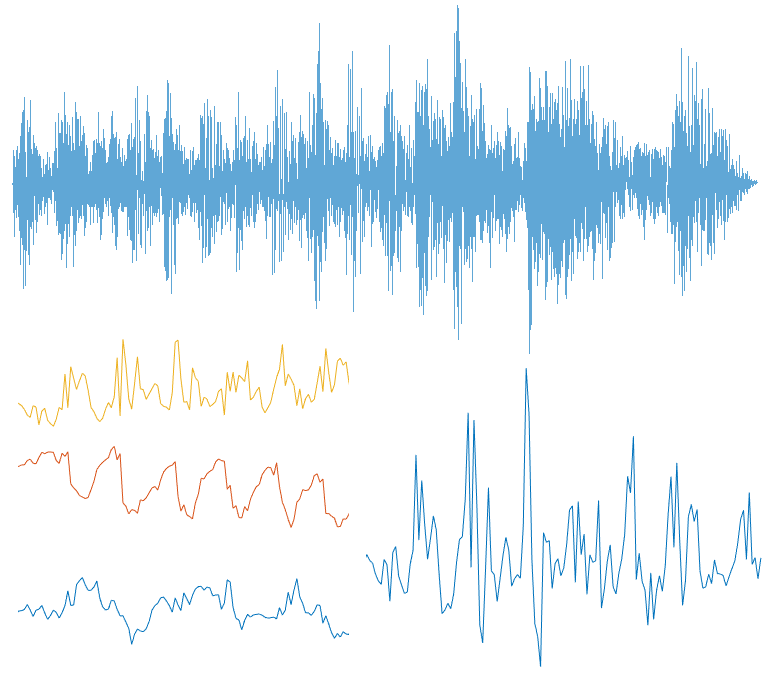
\includegraphics[width=0.9\linewidth]{app_example.png}
			\end{figure}
		\end{minipage}
		
\end{frame}
%--------------------------------------------------------------------------------
\begin{frame}{Литература}
	\begin{enumerate}
		{ \footnotesize
		\item Wang W. et al. Human activity recognition using smart phone embedded sensors // \emph{International Joint Conference on Neural Networks}. 2014.
		\vfill
		\item Kwapisz, Jennifer R., Gary M. Weiss, and Samuel A. Moore. Activity recognition using cell phone accelerometers. // \emph{ACM SigKDD Explorations Newsletter}. 12(2): 74-82. 2011.
		\vfill
		\item Кузнецов М. П., Ивкин Н. П. Алгоритм классификации временных рядов акселерометра по комбинированному признаковому описанию~// \emph{Машинное обучение и анализ данных.} 1(11): 1471-1483. 2015.
		\vfill
		\item Karasikov M. E., Strijov V. V. Feature-based time-series classification // \emph{Intelligence.} 24(1): 164-181. 2016.
		\vfill
		\item Motrenko, A. P., Strijov V. V. Extracting fundamental periods to segment human motion time series // \emph{Journal of Biomedical and Health Informatics.} 2015.
		}
	\end{enumerate}
	
\end{frame}
%--------------------------------------------------------------------------------
%\section{Problem Statement}
\begin{frame}{Постановка задачи}
	\textbf{Заданы} $s \in \mathcal{S}$~--- объект сложной структуры;\\
	\hspace{43pt}$y \in Y$~--- метка класса;\\
	\hspace{43pt}$\mathfrak{D} = \{(s_i, y_i)\}_{i=1}^m$~--- размеченная выборка. \\
	\vfill
	\begin{block}{Задача}
	 Определить функцию $f^*$ такую что 
	 \vspace{-0.2cm}
	 \[
	 f^* = \arg \min_f L\left(f, \mathfrak{D}\right),\vspace{-0.3cm}
	 \] 
	 где $L(\cdot, \cdot)$~--- функция ошибки и $f: \mathcal{S} \rightarrow Y$.
	\end{block}
	\vfill
	\begin{block}{Предположение}
		Предположим что $f = g \circ h$, где
		\begin{enumerate}
			\item $h(s): \mathcal{S} \rightarrow H \subset \mathbb{R}^n$ отображение из $\mathcal{S}$ в признаковое пространство $H$;
			\item $g(\bm{h}, \bm\theta): H \rightarrow Y$ параметрическое отображение (модель классификации).
		\end{enumerate}
	\end{block}
\end{frame}
%--------------------------------------------------------------------------------
\begin{frame}{Оптимальные параметры}
	\begin{minipage}[t]{0.15\columnwidth}
		\vspace{-0.6cm}
		\begin{block}{}
			\centering
			\vspace{0.5cm}
			$\,\,h(s)$
			\vspace{0.5cm}
		\end{block}
	\end{minipage}	
	\hfill
	\begin{minipage}[t]{0.8\columnwidth}
			Выбор функции $h(s)$ обсуловлен
			\begin{itemize}
				\item априорными (экспертными) знаниями;
				\item \textit{минимизацией функционала ошибки.}
			\end{itemize}
	\end{minipage}
\vfill
	\begin{minipage}[t]{0.15\columnwidth}
		\vspace{-0.6cm}
		\begin{block}{}
			\centering
			\vspace{1.5cm}
			$\,\,g(\bm{h}, \bm\theta)$
			\vspace{1.5cm}
		\end{block}
	\end{minipage}	
	\hfill
	\begin{minipage}[t]{0.8\columnwidth}
			Классификация $\{(\bm{h}_i , y_i)\}_{i=1}^m$, $\bm{h}_i = h(s_i)$:
			\[
				\bm{\theta}^* = \arg \min_{\bm\theta} L(g, \bm\theta, \mathfrak{D}),
			\]
		\vspace{-0.3cm}
		\begin{itemize}
		\item $g(\mathbf{h}, \bm\theta)$ - модель классификации;
		\item $\bm\theta$ - параметры модели;
		\item $L (g, \bm\theta, \mathfrak{D})$ - функция ошибки классификации.
		\end{itemize}
	\begin{block}{}
	\[
	\begin{CD} s@>h(\cdot)>> \bm{h} @>g(\cdot, \bm{\theta})>> y
	\end{CD}
	\]
	\end{block}
	\end{minipage}	

\end{frame}
%--------------------------------------------------------------------------------
\begin{frame}{Пример временного ряда}
	\begin{figure}[h]
		\centering
		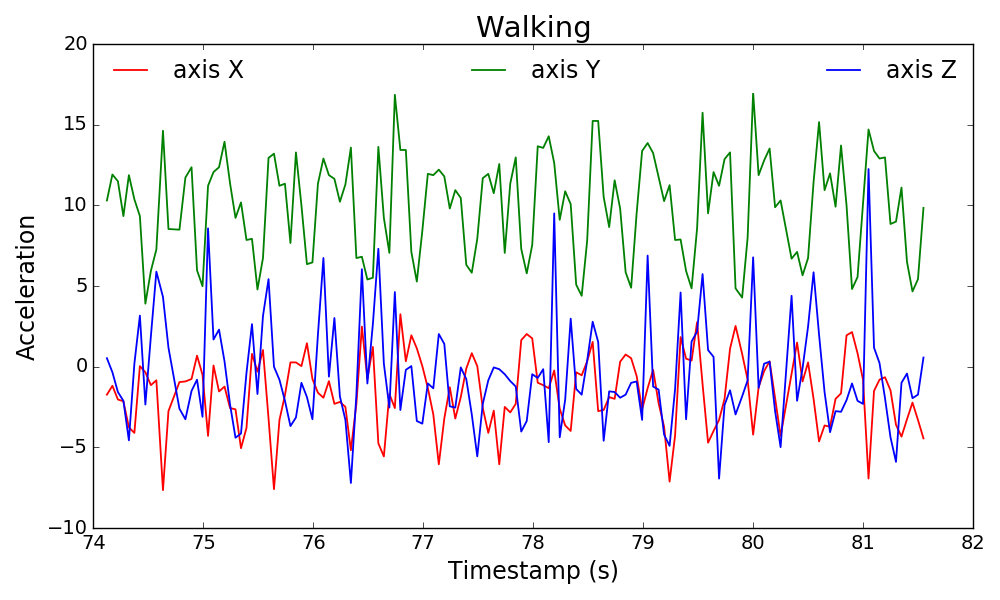
\includegraphics[width=1\linewidth]{ts_example.png}
		\label{ts_example}
	\end{figure}
\end{frame}
%--------------------------------------------------------------------------------
%\section{Feature extraction}
\begin{frame}{Экспертные функции}
	\textbf{Априорное знание} об объектах позволяет извлечь признаки.
	\vfill
	\begin{block}{Признаковое описание}
		$\bm{h}_i = h\left(s_i\right)\in \mathbb{R}^{40}$~--- различные статистики:
		
		\hspace{0.5cm}\fbox{{\scriptsize 3}}$\:\,$ среднее ускорение по каждой оси;\\
		\hspace{0.5cm}\fbox{{\scriptsize 3}}$\:\,$ стандартное отклонение;\\
		\hspace{0.5cm}\fbox{{\scriptsize 3}}$\:\,$ среднее абсолютное отклонение;\\
		\hspace{0.5cm}\fbox{{\scriptsize 1}}$\:\,$ среднее ускорение;\\
		\hspace{0.5cm}\fbox{{\scriptsize 30}} значение гистограммы для каждой оси.
	\end{block}
	\vfill
	\textbf{Проблема:} необходимы экспертные знания.

\end{frame}
%--------------------------------------------------------------------------------
\begin{frame}{Авторегрессионная модель}
	\textbf{Гипотеза порождения данных}
	
		Предположим, что $s = (x_1, \dots, x_\T)$ порождён с помощью авторегрессионной модели:
		\[
			\widehat{x}_t = w_0 + \sum_{j=1}^n w_j x_{t-j}.
		\]
	\vfill
	\begin{block}{Признаковое описание}
		\[
			h(s) = \mathbf{w}^* = \arg \min_{\mathbf{w} \in \mathbb{R}^{n+1}} \sum_{j=n+1}^{T} \left\| x_j - \hat{x}_j \right\|^2.
		\]
	\end{block}
\end{frame}
%--------------------------------------------------------------------------------
\begin{frame}{Анализ сингулярного спектра (SSA)}
	
	\textbf{Траекторная матрица} временного ряда $s = (x_1, \dots, x_\T)$:
	
	\begin{minipage}[t]{0.56\columnwidth}
	\[
		\mathbf{X} = 
		\begin{pmatrix}
			x_1 & x_2 & \dots & x_n \\
			x_2 & x_3 & \dots & x_{n+1} \\
			\vdots & \vdots & \ddots & \vdots\\
			x_{\T-n+1} & x_{\T-n+2} & \dots & x_{\T}
		\end{pmatrix}
	\]
	\end{minipage}
	\begin{minipage}[t]{0.38\columnwidth}
		\begin{figure}
			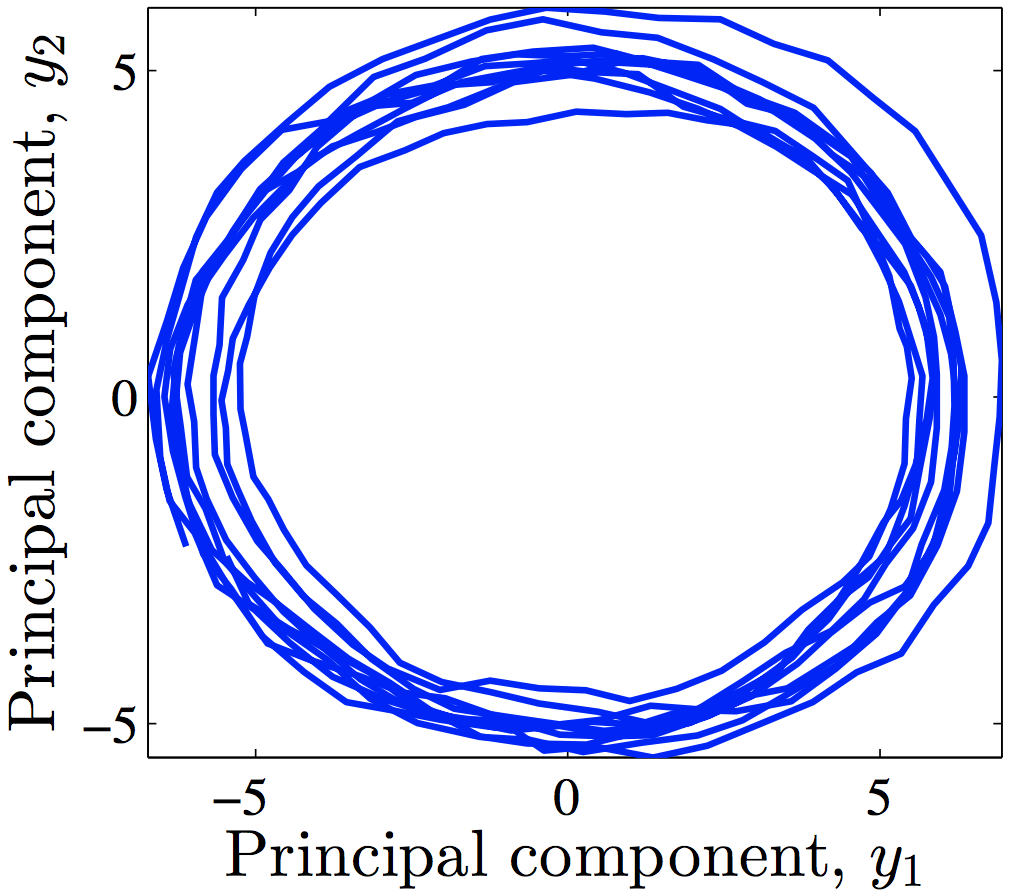
\includegraphics[width=.8\linewidth]{ssa}
		\end{figure}
	\end{minipage}
	\vfill
	\begin{block}{Признаковое описание}
		\[
			h(s) = \left(\lambda_1, \dots ,\lambda_n\right),
		\]
		где $\{\lambda_i\}_{i=1}^n$~--- собственные значения матрицы $\mathbf{X}^{\T} \mathbf{X}$, полученные с помощью SVD:
		$
			\mathbf{X}^{\T} \mathbf{X} = \mathbf{V} \cdot \text{diag} (\lambda_1, \dots, \lambda_n) \cdot \mathbf{V}^{\T}.
		$
	\end{block}
\end{frame}
%--------------------------------------------------------------------------------
\begin{frame}{Кубические сплайны}
	\begin{figure}[h]
		\centering
		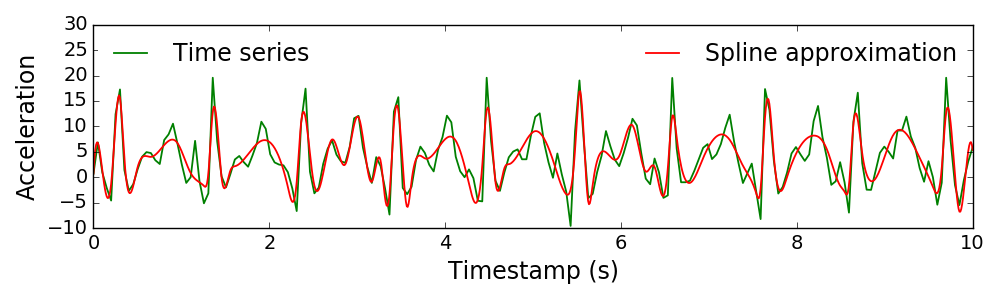
\includegraphics[width=1\linewidth]{spline_example.png}
	\end{figure}
	\vfill
	\textbf{Сплайн} определяется $\{\xi_\ell\}_{\ell=1}^L$~--- набором узлов и\\ \hspace{3.85cm}$\{\mathbf{w}_\ell\}_{\ell=1}^L$ ~--- параметрами моделей, \\ \hspace{3.8cm} построенными на отрезках $[\xi_\ell; \xi_{\ell + 1}]$.
	\vfill
	\begin{block}{Признаковое описание}
		\[
		\bm{h} = h(s) = (\xi_1, \dots, \xi_L, \mathbf{w}_1, \dots, \mathbf{w}_L).
		\]
	\end{block}
\end{frame}
%--------------------------------------------------------------------------------
\begin{frame}{Данные}
\noindent
\begin{minipage}[t]{0.45\linewidth}
	\textbf{WISDM}$^1$
	\begin{table}[]
		\scriptsize
		\label{my-label}
		\begin{tabular}{l|rr}
			\hline
			\textbf{Activity}   & \multicolumn{2}{l}{\textbf{\# objects}} \\
			\hline
			Standing   & 229 & 5.3\% \\
			Walking    & 1917 & 44.4\%\\
			Upstairs   & 466 &10.8\%\\
			Sitting    & 277  &6.4\%\\
			Jogging    & 1075 &24.9\%\\
			Downstairs & 357 &8.3\%\\
			\hline
			Total & \multicolumn{2}{l}{4321}  \\
			\hline
		\end{tabular}
	\end{table}

	\vspace{1cm}
	\medskip\hrule\medskip
	{\scriptsize $^1$http://www.cis.fordham.edu/wisdm/ \\
		$^2$http://sipi.usc.edu/HAD/}
	
\end{minipage}
\hspace{-0.65cm}
\begin{minipage}[t]{0.02\columnwidth}
	\vspace{0.78cm}
	\begin{figure}[h]
		\centering
		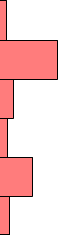
\includegraphics[width=2.3\linewidth]{hist1.png}
	\end{figure}
\end{minipage}
\hfill
\begin{minipage}[t]{0.47\linewidth}
	\textbf{USC-HAD}$^2$
	\begin{table}[]
		\scriptsize
		\label{my-label}
		\begin{tabular}{l|rr}
			\hline
			\textbf{Activity} & \multicolumn{2}{l}{\textbf{\# objects}} \\ \hline
			Walking-downstairs & 951 & 7\%  \\
			Walking-upstairs        & 1018&7.4\%  \\
			Walking-forward    & 1874&13.8\% \\
			Walking-right        & 1305&9.6\%  \\
			Walking-left        & 1280&9.4\%  \\
			Elevator-up        & 764&5.6\% \\
			Elevator-down        & 763&5.6\%  \\
			Standing           & 1167&8.6\%  \\
			Sitting            & 1294&9.5\%  \\
			Sleeping           & 1860&13.7\% \\
			Jumping        & 495&3.6\%  \\
			Running            & 849&6.2\%  \\ \hline 
			Total              & \multicolumn{2}{l}{13620}\\ 
			\hline
		\end{tabular}
	\end{table}
\end{minipage}
\hspace{-0.24cm}
\begin{minipage}[t]{0.02\columnwidth}
	\vspace{0.78cm}
	\begin{figure}[h]
		\centering
		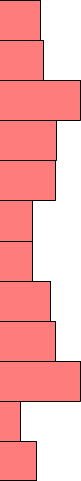
\includegraphics[width=3.135\linewidth]{hist2.png}
	\end{figure}
\end{minipage}

\end{frame}
%--------------------------------------------------------------------------------
\begin{frame}{Эксперимент}
		\begin{align*}
			\text{\textbf{Данные: }} &\text{WISDM, USC-HAD.}\\
		\text{\textbf{Методы генерации признаков: }} &\text{экспертные функции;}\\ &\text{авторегрессионая модель;}\\ &\text{анализ сингулярного спектра;}\\ &\text{сплайны.}\\
		\text{\textbf{Модели классификации:} } &\text{логистическая регрессия;}\\ &\text{SVM;}\\ &\text{случайный лес.}\\
		\text{\textbf{Оптимизация параметров: }} &\text{кросс-валидация.}\\
		\text{\textbf{Метрика качества: }} &\text{точность.}
		\end{align*}

\end{frame}
%--------------------------------------------------------------------------------
\begin{frame}{Результаты}
	\begin{minipage}[t]{0.49\columnwidth}
		\begin{figure}[h]
			\centering
			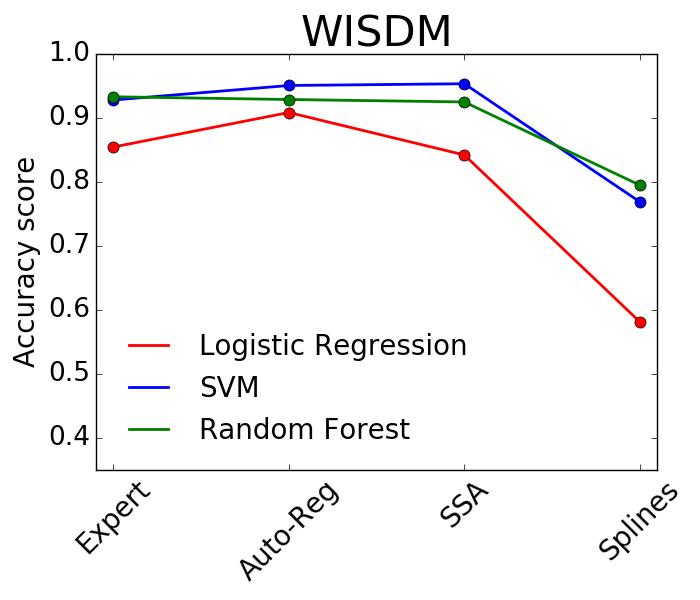
\includegraphics[width=1.05\linewidth]{wisdm_methods.png}
		\end{figure}
	\end{minipage}
	\hfill
	\begin{minipage}[t]{0.49\columnwidth}
		\begin{figure}[h]
			\centering
			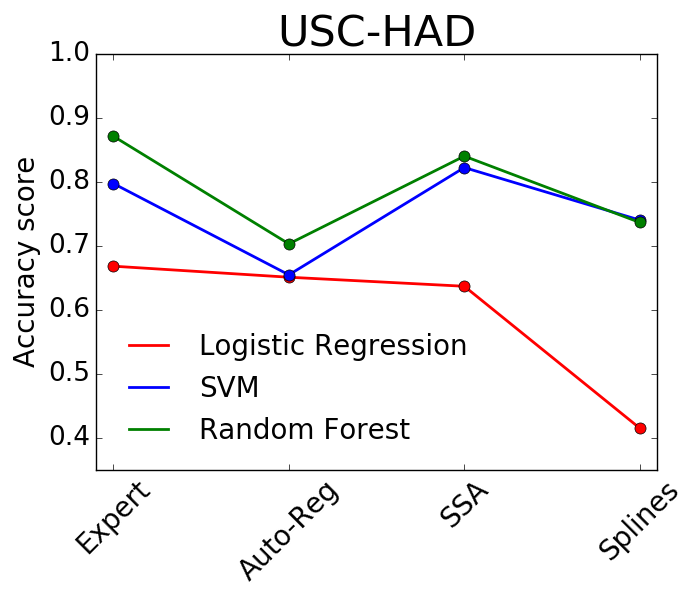
\includegraphics[width=1.05\linewidth]{uschad_methods.png}
		\end{figure}
	\end{minipage}
	\vfill
	\textbf{Объединение всех признаков.}\\
	\vspace{-0.3cm}
	\hspace{1cm}\begin{minipage}[t]{0.39\columnwidth}
		\begin{block}{}
			\centering
			SVM: \textbf{\Large 0.983} 
		\end{block}
	\end{minipage}
	\hspace{1cm}
	\begin{minipage}[t]{0.39\columnwidth}
		\begin{block}{}
			\centering
			Случайный лес: \textbf{\Large 0.882}
		\end{block}
	\end{minipage}
	
\end{frame}
%--------------------------------------------------------------------------------
\begin{frame}{Результаты}
	\textbf{\color{blue} USC-HAD}
	\begin{figure}
		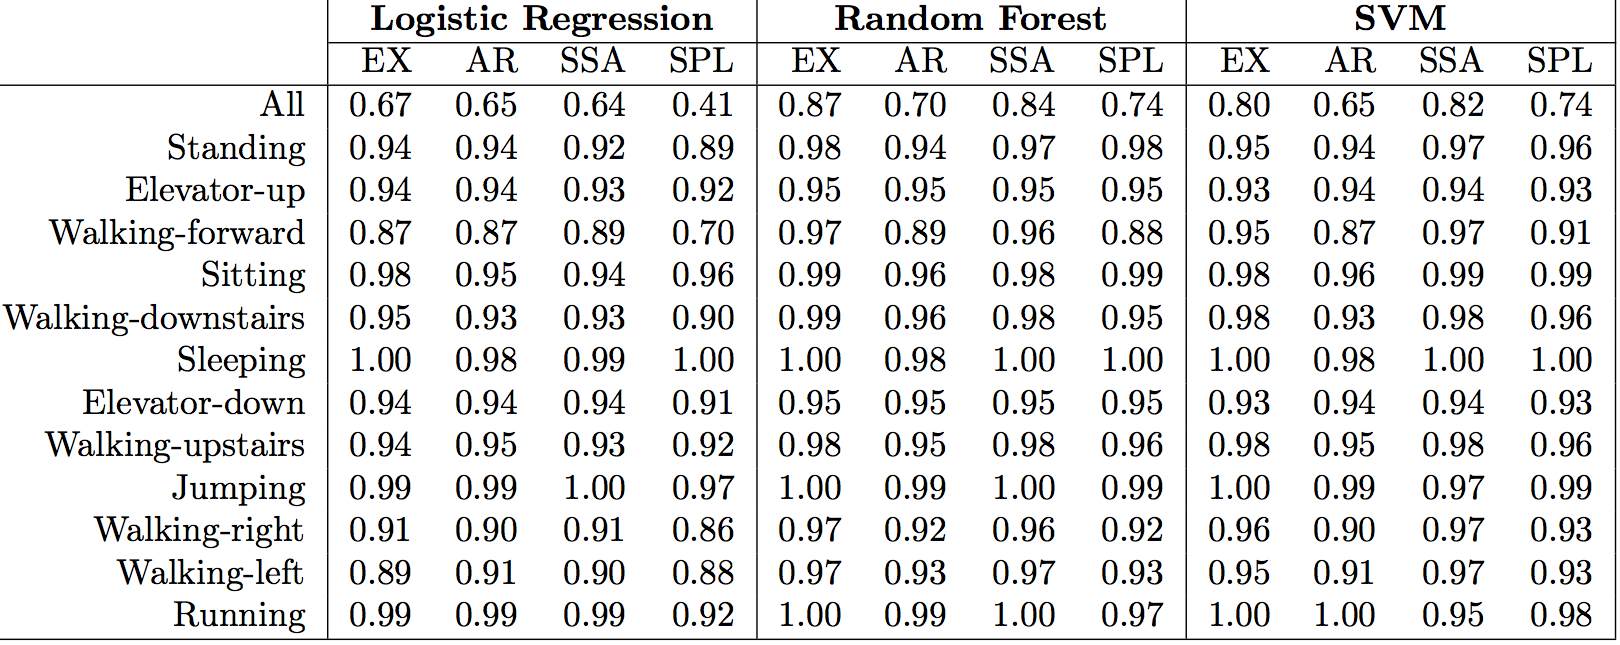
\includegraphics[width=1.\linewidth]{res_numbers}
	\end{figure}
\end{frame}
%--------------------------------------------------------------------------------
\begin{frame}{Результаты}
	\textbf{\color{blue} USC-HAD, объединение признаков}
\begin{figure}[h]
	\centering
	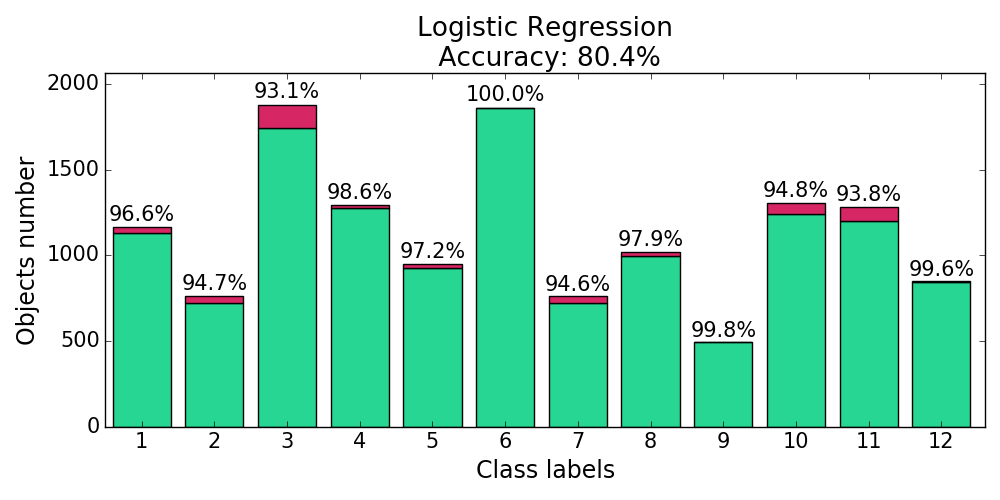
\includegraphics[width=1.0\linewidth]{hist_uschad_lr_all}
\end{figure}
\end{frame}
%--------------------------------------------------------------------------------
\begin{frame}{Выводы}
		\begin{itemize}
			\item задача классификации объектов сложной структуры может быть декомпозирована на две процедуры: извлечения признаков и обучение модели;
			\vfill
			\item параметры локальных моделей могут быть использованы в качестве признакового описания для объектов сложной структуры;
			\vfill
			\item вычислительные эксперименты на реальных данных акселерометра подтвержают гипотезу о применимости подхода.
		\end{itemize}
\end{frame}


\end{document} 